\documentclass[12pt]{article}

\usepackage{graphicx}
\usepackage{fullpage}
\usepackage[utf8]{inputenc}
\usepackage[brazil]{babel}
\usepackage{amsmath}

\begin{document}

\begin{center}
\Large{DCC04 -- Binary Search Trees I}
\end{center}

\vspace{1cm}

\noindent
Nome: \rule{8cm}{0.01in} \ Matr\'{i}cula: \rule{3cm}{0.01in}

\vspace{1cm}

%%%%%%%%%%%%%%%%%%%%%%%%%%%%%%%%%%%%%%%%%%%%%%%%%%%%%%%%%%%%%%%%%%%%%%%%%%%%%%%%

\begin{enumerate}

\item Assume that a binary search tree \texttt{Tree} contains the following
operations:

\begin{itemize}
\item \texttt{typedef struct Node *Tree}

\item \texttt{Reg* getReg(Tree t)}

\item \texttt{Tree getL(Tree t)}

\item \texttt{Tree getR(Tree t)}
\end{itemize}

Thus, any pointer \texttt{t}, having type \texttt{Tree}, is either \texttt{NULL},
or it is a tree-node.
In the latter case, we have the following properties:

\begin{itemize}
\item any element in the left subtree (\texttt{getL}) is less than the 
current element;
\item any element in the right subtree (\texttt{getR}) is greater than the 
current element;
\end{itemize}

From these observations, you must implement a number of algorithms, as requested
below:

\begin{enumerate}
\item Implement a function \texttt{int getHeight(t)}, that returns the height of
any pointer \texttt{t}.
This height is the longest path from \texttt{t} until \texttt{NULL}.

\vspace{5cm}

\item Implement a function \texttt{int getMax(t)}, that returns the largest
element stored in the tree rooted at \texttt{t}.

\vspace{5cm}

\item Implement a function \texttt{int getDiameter(t)}, which returns the
{\em diameter} of the tree \texttt{t}.
The diameter of a tree is the largest distance between two \texttt{NULL} nodes
in the tree.

\vspace{5cm}

\item Implement a function \texttt{int shortestInterval(t)}, which returns the
least difference between two keys stored in \texttt{t}.
For instance, in the tree below, this difference is 3:

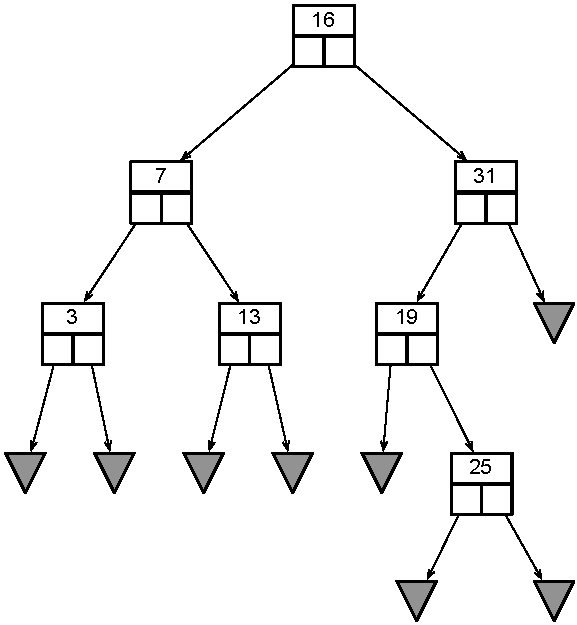
\includegraphics[scale=0.7]{images/binSearchTree_1}

\end{enumerate}

\end{enumerate}

\end{document}
